\chapter{Basics of ergodic information theory}

\section{Stochastic processes and properties of the measure}
We can now go back to the discussion in \cref{par:measure_spaces} and state some useful and insightful results.
\\First of all, recall that we are dealing now with the space of all infinite sequences of our finite alphabet, $\Omega = \mathcal{A}^{\nb}$. We introduced earlier a measure $\mu$ on this space and defined the marginals of our measure as the functions $\mu\big( [x_1^n] \big) = \mu(x_1 ,\dots, x_n, \dots) \equiv \mu_n$ acting on the so called canonical cylinders. Most of the time, we will be working with the so called \textit{stochastic processes}.
\begin{definition}[Stochastic Process]
    A stochastic process is an infinite sequence $X \equiv \big\{ X_n \big\} = \big\{ X_1, X_2, \dots, X_n, \dots \big\}$ of random variables $X_n$ with values in $\alp$, defined by the $k-$th order joint distribution on $\alp^k$:
    \begin{equation*}
        \mu_k(a_1^k) \equiv \mathbb{P} \big( X_1^k = a_1^k \big) \, , \quad a_1^k \in \alp^k
    \end{equation*}
\end{definition}
Equivalently, the distribution of a stochastic process can be completely defined by means of the conditional probabilities, by starting from the one-character distribution $\mu_1$ and then computing the successive conditional distributions:
\begin{equation}
    \mu(x_n|x_1^{n-1}) = \frac{\mu_n(x_1^n)}{\mu_{n-1}(x_1^{n-1})}
\end{equation}
since we could iterate the formula to get 
\begin{equation*}
    \mu(\omega_1, \dots, \omega_n) = \mu(\omega_1) \mu(\omega_2|\omega_1)\mu(\omega_3|\omega_2\omega_1) \dots \mu(\omega_k|\omega_1 \dots \omega_{k-1}) \dots \mu(\omega_n|\omega_1 \dots \omega_{n-1}) 
\end{equation*}
The process $\mu$ is said to be \textbf{\textit{stationary}} if 
\begin{equation}
    \mu(x_1^k) = \mu(x_{n+1}^{n+k}) \: \forall a \in \alp
\end{equation}
We can consider now some dynamics on our probability space $(\Omega, \mathscr{B}, \mu)$, i.e. we consider a transformation $T: \Omega \longrightarrow \Omega'$, where $(\Omega', \mathscr{B}', \mu')$ is another probability space. Most of the times we will actually consider simply consider $\Omega' = \Omega, \mu' = \mu, \mathscr{B}' = \mathscr{B}$. 
\\A transformation $T: \Omega \longrightarrow \Omega'$ is said to be \textit{measurable} if $T^{-1}(\mathscr{B}') \subset \mathscr{B}$ (i.e. $B' \in \mathscr{B}' \Rightarrow T^{-1}B' \in \mathscr{B}$).
\\A transformation $T: \Omega \rightarrow \Omega$ is \textit{measure preserving} if $\forall A \in \mathscr{B}$ we have $\mu \big( T^{-1}(A) \big) = \mu(A)$. We equivalently say then that $T$ is measure preserving or that $\mu$ is \textit{$T$-invariant}, so that $\mu \circ T^{-1} = \mu$. $\mu \circ T^{-1}$ is sometimes referred to as the "pull-back measure" $T^* \mu$. Since $\Omega$ is compact, we can consider the set of all measures on $\Omega$, 
\begin{equation}
    \mathcal{P} = \big\{ \mu \big| \, \mu \, \text{is a finite measure w/} \, \mu(\Omega) = 1 \big\}
\end{equation}
and also we can define 
\begin{equation}
    \mathcal{P}_I = \big\{ \mu \in \mathcal{P} \big| \, \mu \circ T^{-1} = \mu \big\}
\end{equation}
as the collection of all invariant measures (depending on the dynamics). 
\\There is a natural dynamics on $\Omega$: consider $x= (x_0,x_1, \dots, x_n, \dots), x_j \in \alp$. The \textit{\textbf{shift}} is defined as:
\begin{gather}
    \sigma: \Omega \longrightarrow \Omega\nonumber \\
    \sigma : (x_0,x_1, \dots, x_n, \dots) \longrightarrow (x_1, x_2, \dots, x_n, \dots) 
\end{gather}
Its name should be self explicative: it shifts the sequences (to the left).
\\A \textbf{\textit{process}} or a \textbf{\textit{source}} is a shift-invariant probability measure $\mu$ on the topological space $\alp^{\zb}$. The process is uniquely defined by the joint distribution, and not really by the exact values of the $x_n$'s. 
 The shift is closely related to the property of stationarity of the measure: actually, both properties are equivalent.
\begin{prop}[$\sigma$-invariancy $\Leftrightarrow$ stationarity]
Shift invariance implies stationarity, and viceversa. 
\end{prop}
\begin{proof}
    By definition, $\sigma^{-1}( [x_1^n] ) = \{ z \in \Omega \big| \sigma(z) \in [x_1^n] \} = \bigsqcup_{a \in \mathcal{A}} [a, x_1, \dots, x_n]$.
    Then the proof is straightforward, since
    \begin{equation*}
        \mu(\sigma^{-1}( [x_1^n])) = \mu( [x_1^n]) = \sum_{a \in \mathcal{A}} \mu(a, x_1, \dots, x_n)
    \end{equation*}
\end{proof}
Now we may ask ourselves: what if we take $\mu_{n+1} = \mu\big( [x_1{n+1}] \big)$? What is its measure? Notice that 
\begin{equation*}
    [x_1^n] = \bigsqcup_{a \in \mathcal{A}} (x_1, \dots, x_n, a) \, ,
\end{equation*}
i.e. the disjoint union of all sequences which have an arbitrary $n+1$ letter. Thus we can now state the \textit{consistency relations} (or \textit{compatibility conditions}):
\begin{prop}[Consistency relations]
\label{prop:consistency_rel}
\hfill
\\$\mu$ is a measure on $\Omega$ iff:
    \begin{itemize}
        \item[(1)] $\sum_{a_1, \dots, a_k \in \alp} \mu_k(a_1, \dots, a_k) = 1$
        \item[(2)] $\mu_n(x_1, \dots, x_n, \dots) = \sum_{a \in \mathcal{A}} \mu_{n+1} ((x_1, \dots, x_n, \dots, a)$
    \end{itemize}
iff $\mu$ is shift invariant, 
    \begin{itemize}
        \item[(3)] 
         $\mu_n(x_1, \dots, x_n, \dots) = \sum_{a \in \alp} \mu_{n+1}(a, x_1, \dots, x_n, \dots)$
    \end{itemize}
\end{prop}
We can now state a very important result:
\begin{theorem}[Kolmogorov representation theorem]
    If $\{ \mu_k \}$ is a sequence of measure defining a process then there is a \textbf{unique} probability measure $\mu$ on $\alp^{\nb}$ such that, for each $k \geq 1$ and for each cylinder $x_1^k$
    \begin{equation*}
        \mu\big( [x_1^k] \big) = \mu_k(x_1^k)
    \end{equation*}
\end{theorem}
Basically, this is telling us that not only we can reconstruct the measure from the marginals, but that such measure will be the only one we can define on $\Omega$ given such marginals.

\section{Examples of invariant measures}
Let's see some basic examples of invariant measures.
\subsection{i.i.d. (independent identically distributed variables)}
Assume that we have a set of measures $p_1,p_2, \dots, p_n$ over $\alp$ such that 
\begin{gather}
    p_k : \alp \longrightarrow \rb^+ \nonumber \\ 
    p_k \geq 0 \nonumber \\
    \sum_{a \in \alp} p_k(a) = 1 \quad \forall k 
\end{gather}
Define then 
\begin{equation}
    \mu_n(x_1^n) = \mathbb{P}(x_1, \dots, x_n) = \prod_k p_k(x_k)
\end{equation}
choosing $x_1$ with probability $p_1$, $x_2$ with probability $p_2$ and so on. These marginals satisfy all three conditions; consider the first one for example:
\begin{equation*}
    \sum_{x_{n+1}}\mu(x_1 , \dots, x_{n+1}) = p_1(x_1) p_2(x_2) \dots p_n(x_n) \bigg[ \sum_{x_{n+1}} p_{n+1} (x_{n+1}) \bigg] = \mu(x_1 , \dots, x_n)
\end{equation*}
\textit{exercise:} prove that $\forall p_1, \dots, p_n$:
\begin{itemize}
    \item[i)] $\mu = \bigotimes_{j=1}^{\infty}p_j \in \mathcal{P}(\Omega)$
    \item[ii)] $\mu \in \mathcal{P}_I(\Omega) \Leftrightarrow p_k = p : \alp \rightarrow \rb^+ \, \forall k$
\end{itemize}
\subsection{Markov processes}
Markov processes are the easiest stochastic processes with memory. Their definition is quite straightforward:
\begin{definition}[Markov of order $k$]
    \hfill \\
    A process is said to be Markov of order $k$ if
    \begin{equation}
        \mathbb{P}(x_n = a_n \big| x_1^{n-1}) = \mathbb{P}(x_n = a_n \big| x_{n-k}^{n-1}) , \quad n>k
    \end{equation}
    A Markov process of order $1$ is called a Markov chain, i.e. a process is a Markov chain if 
    \begin{equation}
         \mathbb{P}(x_n = a_n \big| x_1^{n-1}) = \mathbb{P}(x_n = a_n \big| x_{n-1}) 
    \end{equation}
\end{definition}
Markov processes have been studied in the past decades to a great extent. We can completely describe a Markov process. To do such thing we have to introduce some objects which simplify our description.
\\First of all, let $\alp = \big\{ a_1, \dots, a_l \big\}$ be our alphabet, with $|\alp| = l$. In a Markov process, the $a_k$'s are called \textit{states}. Consider then a probability vector 
\begin{gather}
    p = (p_1, \dots, p_l) \nonumber \\
    p_j \geq 0 \, , \, \sum_{j=1}^l p_j = 1
\end{gather}
Let then $P = [p_{ij}]$ be a \textit{stochastic} $l \times l$ \textit{matrix} , i.e.
\begin{gather} 
\label{eq:stochastic_matrix}
    P_{ij} \geq 0 \nonumber \\
    \sum_j P_{ij} = 1 \quad \forall j
\end{gather}
The elements of such matrix represent the probability that from a state $i$ we will transition to a state $j$ in the next iteration of our system, i.e. is a matrix representing transition probabilities. That is why the second condition in eq. (\ref{eq:stochastic_matrix}) exists: it is telling us that the probability to transition from a state $i$ to any of the other states $j$ should be $1$.
\\It can be proven that if $P$ is stochastic, then it has an invariant vector $\vec{1}$ of all ones
\begin{equation*}
    P \vec{1} = 
    \begin{pmatrix}
        1 \\
        1 \\
        \vdots \\
        1
    \end{pmatrix}
\end{equation*}
The Perron-Frobenius theorem \cref{par:perron_frobenius_theory} tells us then that all other eigenvalues are contained in a circle of radius $1$. 
\\A Markov process is thus defined by a couple $\big( p, P \big)$. $p$ is invariant if it is a left-eigenvalue
\begin{equation*}
    p P = p \quad (\Leftrightarrow P^T p = p)
\end{equation*}
What measure should we use for a Markov process? A natural definition is, $\forall n$, $ \forall x_1, \dots, x_n $, would be 
\begin{equation}
\label{eq:markov_measure}
    \mu_n(x_1, \dots, x_n) \equiv p(x_1) \cdot P_{x_1 x_2} \cdot P_{x_2 x_3} \cdots P_{x_{n-1} x_n} 
\end{equation}
\begin{prop}
    The measure $\mu$ defined by such marginals satisfies all the consistency relations \ref{prop:consistency_rel}
\end{prop} 
\begin{proof}
\hfill 
    \begin{itemize}
        \item[i)] From their definition (\ref{eq:markov_measure}), $\forall (x_1, \dots, x_n) \in \alp^n$ we have $\mu_n \geq 0$; also since $p$ is a probability vector and $P$ a stochastic matrix we will have $\forall n$ that $\sum_{(x_1, \dots, x_n) \in \alp^n} \mu_n (x_1, \dots, x_n) = 1 $ 
        \item[ii)] The second property $\sum_{x_{n+1}} \mu_{n+1} (x_1, \dots, x_{n+1}) = \mu_n (x_1, \dots, x_n)$ also follows from the definition (\ref{eq:markov_measure}) and stochasticity of $P$
        \item[iii)] The only thing left to prove is that $\sum_{x_0} \mu_{n+1} (x_0, x_1, \dots, x_n) =  \mu_n (x_1, \dots, x_n)$. This is actually straightforward since 
        \begin{equation*}
            \sum_{x_0} p_{x_0} P_{x_0 x_1} P_{x_1 x_2} \cdots P_{x_{n-1} x_n} = p(x_1) P_{x_1 x_2} \cdots P_{x_{n-1} x_n}
        \end{equation*}
        where we used the fact that $p$ is an eigenvector of $P$ and thus $(pP)_{x_1} = p_{x_1}$
    \end{itemize}
\end{proof}
By Kolmogorov we then know that this is the unique invariant measure we can define on a Markov process $(p, P)$.
\\An interesting and useful fact is that a markov of order $k$ can always be reduced to order $1$ by using a bigger alphabet (whose cardinality grows exponentially though, so that this becomes difficult to implement in concrete problems). Let's consider for example a Markov of order $2$, 
\begin{equation*}
    \mu (x_1, \dots, x_n \big| x_{n+1}) = \mu (x_1, \dots, x_n) \mu (x_{n+1} \big| x_1, \dots, x_n) = \mu (x_1, \dots, x_n \big| x_{n+1}x_n)
\end{equation*}
Now consider 
\begin{equation*}
    \alp^{(2)} = \big\{ a_ja_k \equiv b \big| 
    \begin{matrix}
        a_j \in \alp \\
        a_k \in \alp
    \end{matrix}
    \big\}
\end{equation*}
as the set of all bigrams. Of course if $\mu$ is a Markov of order $2$ on $\alp$ it can be seen as a Markov Chain on $\alp^{(2)}$.
\\Consider now a Markov chain over $\alp$ with $|\alp| = l$; it may happen that some elements of $P$ are zero, for example consider
\begin{gather*}
    p_j > 0 \quad j=1, \dots, k \\
    p(a_j) = 0 \quad j=k+1, \dots, l
\end{gather*}
we can then reduce this to a Markov chain over $\alp^k$, a smaller alphabet, just erasing rows and column of $P$ to get a new $\hat{P}$ which will be $k \times k$, 
\begin{equation*}
    (p,P) \, \, \text{on} \, \, \alp^l \longrightarrow (\hat{p},\hat{P}) \,\, \text{on} \,\, \alp^k
\end{equation*}

\subsection{Hidden Markow Models}
A hidden Markov model (HMM) is a statistical Markov model in which the system being modeled is assumed to be a Markov process with unobservable ("hidden") states.
\\Let's consider two alphabets: 
\begin{align}
    &\alp = \big\{ x_1, \dots, x_n \big\} \quad \text{observable states} \nonumber \\
    &\mathcal{L} = \big\{ y_1, \dots, y_l \big\} \quad \text{hidden states}
\end{align}
We assume that there exists a rectangular stochastic matrix $R$ such that
\begin{gather}
    R = [R_{yx}]_{y \in \mathcal{L}, \, x \in \alp} \nonumber \\
    \sum_{x \in \alp} R_{yx} = 1 \quad \forall y \in \mathcal{L}
\end{gather}
The elements of $R$ represent the so called \textit{emission probabilities}, i.e. the probabilities to go from an hidden state $y \in \mathcal{L}$ to an observable state $x \in \alp$. Summing on all observable states should amount to $1$ since from an hidden state we must go to some observable state sooner or later (see Fig. \ref{fig:HMM1}). 
\\Surely, we must also assume that there exists also a stochastic matrix for the hidden states with their transition probabilities: this would be the $l \times l$ matrix $P = [P]_{y z}$ $\forall y,z \in \mathcal{L}$. We shall also consider a probability vector $p$ for this Markov system. An HMM is thus defined by a triplet $\big(p, P, R \big)$
\\Then we define the measure for this system as 
\begin{equation}
    \mu_n (x_1, \dots, x_n) = \sum_{(y_1, \dots, y_l) \in \mathcal{L}} p_{y_1} R_{y_1 x_1} P_{y_1 y_2} R_{y_2 x_2} \cdots P_{y_{n-1} y_n} R_{y_n x_n}
\end{equation}
\textit{exercise}:
\begin{itemize}
    \item[i)] prove that $\mu_n$ are marginals (they statisfy the first $2$ consistency relations)
    \item[ii)] prove that if $pP=p$ then $\mu$ is invariant 
\end{itemize}
There is an equivalent way of defining such measure: we can consider the matrix $M_x$ $\forall x \in \alp$ defined as 
\begin{equation}
    M_x = [m_{yz}^{(x)}]_{y, z \in \mathcal{L}} = \big[ R_{yx} P_{yz} \big]
\end{equation}
so that $P = \sum_{x \in \alp} M_x$. These are again $l \times l$ matrices, and there are $n = |\alp|$ of them.
\\This gives us an equivalent representation of an HMM, since considering a probability vector $p = (p_1, \dots, p_l)$ we can define the marginals as 
\begin{equation}
    \mu_n (x_1, \dots, x_n) \equiv p M_{x_1} M_{x_2} \cdots M_{x_n} \cdot 
    \begin{pmatrix}
        1 \\
        1 \\
        \vdots \\
        1
    \end{pmatrix} 
    \,\, \geq 0
\end{equation}

\begin{figure}[h]
    \centering
    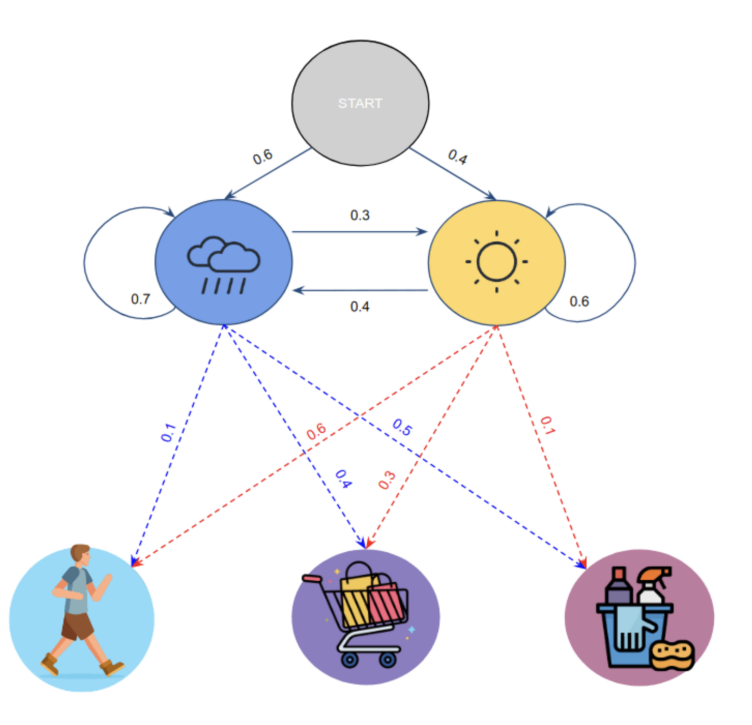
\includegraphics[width=7cm]{img/HMM1.png}
    \caption{Schematic representation of an Hidden Markov Model. My friend lives in the States. Depending on the weather there, he chooses the activity he does every day. I am not able to know the weather where he lives (hidden states), I only know what he is doing that day (observable states).}
    \label{fig:HMM1}
\end{figure}

\section{Ergodic Theory}
We shall now look at some basics results of Ergodic Theory.
\\Consider a space $\man$ with a measure $\mu$ and a certain dynamic $T$ which is measure preserving. Such transformation could be either discrete or continuous (a so called \textit{flow} $\Phi^t$). Given an $x_0 \in \man$ we are interested in studying the orbit under $T$, i.e. all the points $\mathcal{O}(x) = \big\{ x \in \man \big| \, x_n = T^n(x_0), \, \forall n \in \nb \big\}$. 
\\The first thing that comes natural to study are functions from $\man $ to $\rb$, out \textit{observables} $f: \man \longrightarrow \rb$. 
\\We are interested in knowing the asymptotic statistical properties of such observables, i.e. we would like to know for each $f$ what happens to the average
\begin{equation*}
    \lim_{n \rightarrow \infty} \frac{f(x_0) + f(x_1) + \dots + f(x_n)}{n} = \lim_{n \rightarrow \infty} \frac{1}{n} \sum_{k=0}^{n-1} f \circ T^k(x) \equiv f^*(x)
\end{equation*} 
\begin{remark}
    equivalently for flows we could consider 
    \begin{equation}
        \frac{1}{T} \int_0^T (f \circ \Phi^t) (x) \, d\mu
    \end{equation}
    and then take the limit for $T \rightarrow \infty$
\end{remark}
Let's then define the spatial mean of a function $f$, if it exists, as 
\begin{equation}
    \Bar{f} = \int_{\man} f(x) \, d\mu
\end{equation}
A very important classical result is Birkhoff Ergodic Theorem.
\begin{theorem}[Birkhoff Ergodic Theorem]
    Let $(\man, T, \mu)$ be a dynamical system, and $f \in L^1 \big( \man, \mu \big)$ a summable function with complex values. Then 
    \begin{itemize}
        \item[a)] $f^* (x)$ exists $\mu$-almost everywhere
        \item[b)] $f^* (x)$ is summable and invariant almost everywhere, i.e. 
        \begin{equation*}
            f^* (T^k (x) ) = f^*(x) \quad \forall k \, \, \text{a.e.}
        \end{equation*}
        \item[c)] 
        \begin{equation*}
            \int_{\man} f^*(x) \, d\mu = \int_{\man} f \, d\mu
        \end{equation*}
    \end{itemize}
\end{theorem}
Let's define a particular class of functions which will be very useful:
\begin{definition}[Characteristic functions]
    The characteristic function of an open set $A \in \man$ is defined as 
    \begin{equation}
    \chi_A (x) = 
        \begin{cases}
            1 \quad & \text{if} \quad x \in A \\
            0 \quad & \text{if} \quad x \notin A
        \end{cases}
    \end{equation}
\end{definition}
\textit{exercise:} prove that $\chi_A \circ T = \chi_{T^{-1}(A)}$, $\, \forall x \in \man$. 
\begin{prop}
    The following are equivalent:
    \begin{itemize}
        \item[a)] $\forall f \in L^1$, $f^*=c$ $\mu-$a.e.
        \item[b)] $\forall f \in L^1$, $f^*= \int_{\man} f \, d\mu = \Bar{f}$
        \item[c)] if $f \in L^1$ is invariant $\Rightarrow f=$constant
        \item[d)] if $A \subseteq \man$, $A$ measurable and invariant $\Rightarrow \mu(A) = 0,1$
    \end{itemize}
\end{prop}
\begin{proof}
\hfill
    \begin{itemize}
        \item a) $\Rightarrow$ b): \\
         if $f \in L^1$ then $\Rightarrow f= $ constant by a). By point $b$ of Birkoff's theorem we have then 
         \begin{equation*}
             \int_{\man} c \, d\mu =\int_{\man} f^* \, d\mu = \int_{\man} f \, d\mu
         \end{equation*}
         \item b) $\Rightarrow$ c): \\
         take $f$ to be invariant, i.e. $f \circ T = f$: then $f \circ T^k = f \, \forall k \in \nb \Rightarrow f^* = f$
         \item c) $\Rightarrow$ d): \\
         Apply c) to $f = \chi_A \in L^1$. Since $T^{-1}A = A$ mod$\mu$ $\Rightarrow \chi_{T^{-1}A} = \chi_A$ then we have by c) that $\chi_A =$const. By the definition of $\chi$ then we must have const$=0$ and $A = \emptyset$ or const$=1$ and $A = \man$.
         \item d) $\Rightarrow$ a): \\
         claim : $f: \man \rightarrow \rb$ is constant a.e. iff $\nexists l \in \rb$ such that $\mu( \{ x \in \man | f(x) = l \} ) \in (0,1)$, meaning that we only want $\mu$ to have a single jump from $0$ to $1$ and not multiple jumps.
         \\Consider now $f^*$. Suppose that $\nexists l \in \rb$ s.t. for $A_l = \{ x \in \man | f^*(x) = l \}$ s.t. $\mu (A_l) \in (0,1)$. Clearly $T^{-1}A_l = A_l$. But then 
         \begin{equation*}
             T^{-1}A_l = \{ y \in \man | \, f^* (Ty) \leq l \} = A_l \Rightarrow f^* (Ty) = f^*(y)
         \end{equation*}
         and we get a contradiction.
    \end{itemize}
\end{proof}
Thus ergodicity of a system can be also seen as the \textbf{equivalence of time mean and phase space means} of an observable (which is what Boltzmann had hoped was true for any dynamical system). 
\\We can also say that 
\begin{equation*}
     \text{$\%$ of time spent by $\mathcal{O}(x)$ in $A$} =  \frac{ \# \big\{ k | \, x_k \in A \big\}}{n} \xrightarrow{n \rightarrow \infty} \mu(A) = \frac{\mu(A)}{\mu(\man)}  
\end{equation*}
This follows directly from Birkoff's theorem, since if we consider $\chi_A (x)$ then we'll have 
\begin{equation*}
    \chi^*_A = \lim_{n \rightarrow \infty} \frac{1}{n} \sum_{k=0}^{n-1} \chi_A \circ T^k(x) = \int_{\man} \chi_A \, d\mu
\end{equation*} 
Therefore, \textbf{in an ergodic system all orbits visit volumes in phase space for a time proportional to the volumes themself}. \\
Now we could ask ourselves: how does all the discussion about infinite sequences of finite alphabets relate to ergodic theory and its application? The key to deeply connect both arguments will be \textit{partioning}. 
\\Given our measurable dynamical system $(X, \mu, T)$, consider $X$ as partitioned in disjoint sets $P_a$ indexed by a finite alphabet $\alp$, i.e. consider a finite partition $\mathcal{P}$ of $X$ such that
\begin{gather}
    \mathcal{P} = \big\{ P_a \big\}_{a \in \alp} \nonumber \\
    X = \bigsqcup_{a \in \alp} P_a
\end{gather}
The $P_a$'a only intersect on boundaries (sets of zero measure) as shown in Fig. \ref{fig:partition} 
\begin{figure}[h]
    \centering
    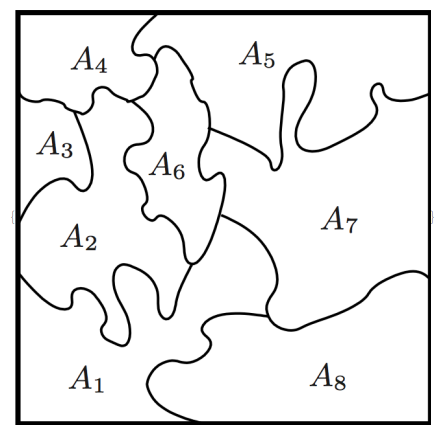
\includegraphics[width=5cm]{img/partition.png}
    \caption{Schematic depiction of a partition of a manifold $X$.}
    \label{fig:partition}
\end{figure}
Then associate each iteration of the dynamics $x_j = T^J(x_0)$ with a given symbol of $\alp$ by the map
\begin{gather*}
    x_1 \longrightarrow \omega_1 \\
    x_2 \longrightarrow \omega_2 \\
    \vdots \\
    x_n \longrightarrow \omega_n \\
    \vdots \\
    \text{where} \quad x_j \in P_{\omega_j}
\end{gather*}
This allows us to equivalently consider an orbit $\mathcal{O}(x)$ or a sequence of characters from our alphabet. 
\\But what measure should we use for such sequences? A marginal $\mu_k(\omega_1^k)$ will now measure all the points which are in $P_{\omega_1}$ at $t_1$, $P_{\omega_2}$ at $t_2$ and so on ($\omega_1$ and $\omega_2$ possibly being the same symbol). Let's define then
\begin{equation}
\label{eq:measure_partition}
    \mu_k (\omega_1^k) = \mu \big( \bigcap_{j=1}^k T^{-j+1} P_{\omega_j} \big)
\end{equation}
\textit{exercise:} prove that such $\mu_k$'s are in fact marginals and that the transformation $T$ commutes with the shift $\sigma$ and that $\mu$ is then $\sigma$- invariant.
\begin{definition}
    The (stationary) process $\{ X_n \}_{n \in \nb}$ defined by the measure (\ref{eq:measure_partition}) is called a $(T, \mathcal{P})$-process
\end{definition}
We can now finally move on to the definition of ergodicity. This comes very naturally by the setting we are now working in. First of all, let's see a couple of definitions needed to state ergodicity:
\begin{definition}
    A measurable set $B \in X$ is said to be $T$-invariant if $TB \subseteq B$
\end{definition}
\begin{definition}
    The space $X$ is said to be $T$-decomposable if it can be expressed as the disjoint union $X = X_1 \bigsqcup X_2$ of two measurable invariant\footnote{since the sets are invariant, the orbit of a point in $X_1$ stays in $X_2$ and the same thing happens for $X_2$. Therefore we could study the two subsystem separately} sets, each of positive measure. Hence, the space is indecomposable if 
    \begin{equation*}
        T^{-1}B = B \Rightarrow \mu(B) = 0 \, \vee \, \mu(B) = 1
    \end{equation*}
\end{definition}
This is exactly what we mean for ergodicity. 
\begin{definition}[Ergodicity]
    A measure-preserving tranformation $T$ is said to be \textbf{ergodic} if
    \begin{equation}
        T^{-1}B = B \Rightarrow \mu(B) = 0 \, \vee \, \mu(B) = 1
    \end{equation}
\end{definition}
Thus \textbf{ergodicity of our system means that we cannot subdivide it in smaller parts to study them separately}.
\\Notice that Hamiltonian systems are not ergodic: we can subdivide them in hypersurfaces where the hamiltonian $H=E$ is constant. 
\begin{lemma}[Ergodicity equivalents]
    The following are equivalent for a $\mu$-measure preserving transformation $T$:
    \begin{itemize}
        \item[1)] $T$ is ergodic
        \item[2)] $T^{-1}B \subseteq B \Rightarrow \mu(B) = 0 \, \vee \, \mu(B) = 1$
        \item[3)] $T^{-1}B \supseteq B \Rightarrow \mu(B) = 0 \, \vee \, \mu(B) = 1$
        \item[4)] $\mu (T^{-1}B \Delta B) = 0 \Rightarrow \mu(B) = 0 \, \vee \, \mu(B) = 1$
        \item[5)] $f \circ T = f$ a.e. $\Rightarrow f$ constant a.e.
    \end{itemize}
\end{lemma}
The last claim can be proved by recalling that $\chi_A \circ T = \chi_{T^{-1}A}$ (\textit{exercise}). 
\\We will see later on what ergodicity of our system means in the setting we discussed earlier. Basically, it will coincide with an application of ergodicity itself, which is the convergence of empirical probabilities. But for now, let's stick to studying some other basic results of ergodic theory.
\\Sometimes, to show that a process is ergodic it is even simpler to prove a stronger property, called \textit{mixing}. 
\begin{definition}[Mixing]
    A measure preserving transformation $T$ is mixing if for any pair of measurable sets $C$ and $D$ we have
    \begin{equation}
        \lim_{n \rightarrow \infty} \mu \big( T^{-n}C \cap D \big) = \mu(C) \cdot \mu(D)
    \end{equation}
\end{definition}
This definition is telling us that the fact that a system is mixing corresponds to the fact that correlations are asymptotically decaying\footnote{we could also have "exponential mixing" or "polynomial mixing" based on how the decay evolves with time ($\sim e^{-t}$ or $\sim t^{-\alpha}$)}. Basically then \textit{a mixing system is a system with no memory}. 
\\\textit{exercise:} prove that mixing $\Rightarrow$ ergodicity (and that the viceversa is not true).
\\Actually, some sort of viceversa of mixing $\Rightarrow$ ergodicity does exist, but with looser conditions: we can say that "mixing on average" $\Rightarrow$ ergodicity, in the following sense:
\begin{theorem}
    The dynamical system $(X, \mu, T)$ is ergodic if and only if $\forall A,B \subset X$ 
    \begin{equation}
        \lim_{n \rightarrow \infty} \frac{1}{n} \sum_{j=0}^{n-1} \mu \big( A  \cap T^{-1}B \big) = \mu(A) \cdot \mu(B)
    \end{equation}
\end{theorem}

\subsection{Ergodicity for Markov chains}
When is a Markov chain irreducible? When we cannot have a zero probability to go from a state $j$ to a state $k$.
\begin{definition}[irreducible Markov chains]
    The stochastic matrix $M$ is said to be irreducible if for any pair $j,k$ there is a certain sequence $j_0, j_1, \dots, j_n$ with $j_0=j$ and $j_n=k$ such that each intermediate transition is possible, i.e. 
    \begin{equation}
        M_{j_m j_{m+1}} > 0 \,, \quad m = 0,1, \dots, n-1
    \end{equation}
    Namely, given any pair of states $j$ and $k$, sooner or later strarting from $j$ we'll end up in $k$.
\end{definition}
This actually corresponds (\textit{exercise: chech it}) to the definition of irreducible matrices given in par. \cref{par:perron_frobenius_theory}, i.e. $\forall i,j$ $\exists n = n(i,j) : (P^n)_{ij} > 0$.
If $M$ is irreducible then by Perron-Frobenius (\cref{par:perron_frobenius_theory}) there is a \textbf{unique} probability vector $\pi$ (the \textbf{equilibrium state}):
\begin{equation}
    \pi M = \pi
\end{equation}
i.e. the Markov chain with start distribution $\mu_1=\pi$ and transition matrix $M$ is in fact a stationary process. 
\\Moreover, any initial distribution of characters will \textit{converge to the invariant measure}: given any probability vector $\mu_1$ on $\alp$, we have 
\begin{equation}
    \lim_{n \rightarrow \infty} \mu_1 M^n = \pi
\end{equation}
We can define the equivalent of the mixing property for a Markov chain:
\begin{definition}
    A Markov chain is mixing iff $\exists$ n s.t. $\forall j,k$ we have $M_{jk}^n$.
\end{definition}
This is a stronger requirement than irreducibility, as we are now asking that such $n$ is not a function of the indexes $i,j$ but instead exists for all couples. This definition of mixing is quite straightforward and equivalent to that given before: let's give it a better look. 
\\Consider a Markov system $(p, P)$ on a space $(\Omega=\alp^{\nb}, \mu, T = \sigma)$. Consider then two cylinders $C= [x_1^m]$ and $D= [y_1^r]$. we know that mixing means for our two sets that 
\begin{equation*}
    \lim_{n \rightarrow \infty} \mu (T^{-n}C \cap D) = \mu(C) \, \mu(D)
\end{equation*}
Of course $T^{-n} = \sigma^{-n}$ is just a translation, i.e. $T^{-n}(C) = \big\{ z \in \Omega | \, z_{n+j} = y_j, \quad j=1, \dots, r \big\}$. What is then $T^{-n}C \cap D$? Consider an $n > m$ for simplicity. Then
\begin{equation*}
    T^{-n}C \cap D = \bigg\{ z \in \Omega \bigg| \, 
    \begin{matrix}
        z_1 = x_1 & z_{n+1} = y_1 \\
        \vdots & \vdots\\
        z_m=x_m  & z_{r+n} = y_r
    \end{matrix}
    \bigg\}
\end{equation*}
The measure of this set in with our Markov measure will then be (see Fig. \ref{fig:markov_line}):
\begin{align}
    \mu(T^{-n}C \cap D) = p_{x_1} P_{x_1 x_2} \cdots P_{x_{m-1} x_m} \cdot \bigg( \sum_{z_1, \dots, z_k} P_{z_1 z_2} \cdots P_{z_{t-1} z_t = y_1} \bigg) P_{y_1 y_2} \cdots P_{y_{r-1} y_r} \nonumber \\
    =  p_{x_1} P_{x_1 x_2} \cdots P_{x_{m-1} x_m} \cdot \big( P^t\big)_{x_m y_1} P_{y_1 y_2} \cdots P_{y_{r-1} y_r}
\end{align}
\begin{figure}[h]
    \centering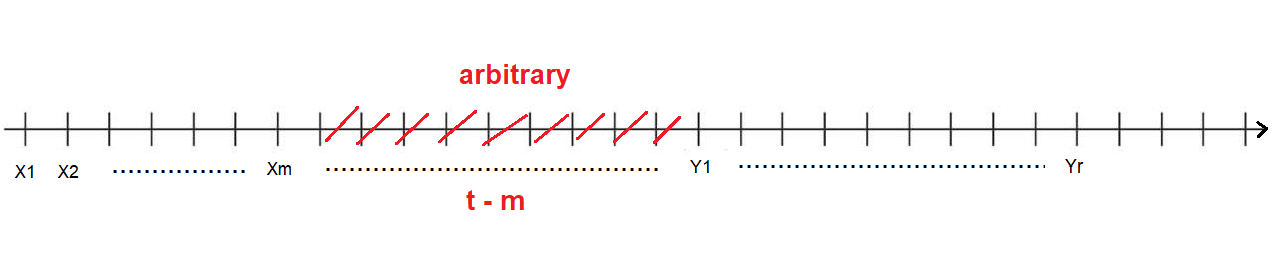
\includegraphics[width=12cm]{img/markov_line.png}
    \caption{Schematic depiction of our Markovian sequences. The sequence from $X_m$ to $Y_1$ is totally arbitrary.}
    \label{fig:markov_line}
\end{figure}
since we must account for all possible paths from $x_m$ to $y_1$ in $t$ steps. 
\\A very useful classical result is the following:
\begin{theorem}[Ergodicity for Markov chains]
\hfill
    \begin{itemize}
        \item[(1)] A stationary Markov chain is ergodic iff its transition matrix $M$ is irreducible
        \item[(2)] If the Markov chain is mixing, then it is ergodic
    \end{itemize}
\end{theorem}
Some more useful results for Markov chains' ergodicity are the following. 
\begin{lemma}{(1.18 in Walter)}
    Let $P$ be a stochastic matrix and $P^n$ its power. Take then a "Birkoff average" of $P$, 
    \begin{equation}
    \label{eq:Q_projector}
        Q = \lim_{n \rightarrow \infty} \frac{1}{n} \sum_{k=0}^{n-1} P^n
    \end{equation}
    Such matrix is a spectral projector, i.e. it satisfies $Q^2 = Q$; moreover, it commutes with $P$, $QP = PQ$ and $\forall v$ such that $vP = v$ we have that $vQ = v$.
\end{lemma}
The existence of $Q$ can be proven by spectral theory. By using $Q$ we can state two theorems which can result useful:
\begin{theorem}
    The following are equivalent:
    \begin{itemize}
        \item[a)] $(\Omega, \mu, T)$ is ergodic;
        \item[b)] $Q$ as defined in (\ref{eq:Q_projector}) is an $l \times l$ matrix of the form 
        \begin{equation*}
            Q = 
            \begin{pmatrix}
                \Vec{p} \\
                \Vec{p} \\
                \vdots \\
                \Vec{p} 
            \end{pmatrix}
        \end{equation*}
        where $p$ is a probability vector (i.e. $pP = p$, $p_j \geq 0$, $\sum_j p_j = 1$)
        \item[c)] $P$ is irreducible
        \item[d)] $\Vec{1}$ s.t. $P \Vec{1} = \Vec{1}$ is a simple eigenvector (but not the only eigenvector).
    \end{itemize}
\end{theorem}
There is an equivalent of the last theorem for mixing:
\begin{theorem}
    The following are equivalent:
    \begin{itemize}
        \item[a)] $(\Omega, \mu, T)$ is mixing;
        \item[b)] $P$ is irreducible and aperiodic
        \item[c)] $P^n \xrightarrow{n \rightarrow \infty} Q$ with 
        \begin{equation*}
            Q = 
            \begin{pmatrix}
                \Vec{p} \\
                \Vec{p} \\
                \vdots \\
                \Vec{p}
            \end{pmatrix}
        \end{equation*}
        \item[d)] $\Vec{1}$ s.t. $P \Vec{1} = \Vec{1}$ is a simple eigenvector \textbf{and} it is the unique eigenvalue on $S^1$ (the circle).
    \end{itemize}
\end{theorem}


\section{Consequences of ergodicity}
\begin{definition}[empirical frequencies]
    Given a sequence $x = x_1^n \in \alp^n$ of length $n$ and a $k$-gram $\omega = \omega_1 \omega_2 \dots \omega_k \in \alp^k$, we define the \textbf{empirical frequency} of the word $\omega$ by 
    \begin{equation}
        f_x(\omega) \equiv | \big\{ j \in [1, n-k+1] : x_j^{j+k-1} = \omega \big\} |
    \end{equation}
\end{definition}
Denoting by $\chi_\omega$ the indicator function of the cylinder $[\omega_1^n]$ we could also write 
\begin{equation}
    f_x(\omega) = \sum_{j=1}^{n-k+1} \chi_\omega (\sigma^{j-1} x)
\end{equation}
Meaning that, since we are looking at how many times a word appears in a sequence, we could do it by sliding a window of size $k$ over our sequence e count a $+1$ for every match. 
\begin{definition}[relative frequency]
    The relative frequency is instead defined as 
    \begin{equation}
        \hat{\mu}_n (\omega_1^k | x_1^n) \equiv \frac{1}{n-k+1} f_x(\omega_1^k)
    \end{equation}
\end{definition}
\begin{definition}[typical sequences]
    A sequence $x \in \alp^{\nb}$ is said to be frequency \textbf{typical} for the process $\mu$ if each word $\omega \in \alp^{\nb}$ appears in $x$ with the statistics predicted by $\mu$, i.e. 
    \begin{equation}
        \lim_{n \rightarrow \infty} \hat{\mu}_n (\omega_1^k | x_1^n) = \mu(\omega_1^k)
    \end{equation}
    The set of all typical sequences is denoted by $\mathcal{T} \subseteq \alp^{\nb}$: 
    \begin{equation}
        \mathcal{T} \equiv \big\{ x \in \alp^{\nb} : x \, \, \,\text{is typical} \big\}
    \end{equation}
\end{definition}
If my system is ergodic and it behaves nicely, then I would expect that if I look at the typical sequence $x$ this should contain $\omega$ with the same proportion given by the invariant measure. We do not expect typically to have a million zeros and a single one from a coin toss with a fair coin. 
\\So, \textbf{an ergodic system would be one for which we can reconstruct} $\mathbf{\mu}$ \textbf{from the data} (all words appear typically). 
\begin{theorem}[Typical-sequence theorem]
    If $\mu$ is ergodic 
    \begin{equation}
        \mu\big( \mathcal{T}(\mu) \big) = 1
    \end{equation}
    that is, for all $\omega \in \alp^{\nb}$
    \begin{equation*}
        \lim_{n \rightarrow \infty} \hat{\mu}_n (\omega_1^k | x_1^n) = \mu(\omega_1^k), \quad \text{for almost every} \, x
    \end{equation*}
\end{theorem}
Note that this coincides with the property of ergodic systems not being decomposable in smaller parts. 
The last theorem is also true in the other way around:
\begin{theorem}[Typical sequence converse theorem]
    Suppose $\mu$ is a stationary measure such that for eah $\omega \in \alp^{\nb}$ the limiting relative frequencies $\hat{\mu}(\omega|x)$ exist and are constant in $x$, $\mu-$almost surely.
    \\Then,
    \begin{center}
        $\mu$ is an ergodic measure
    \end{center}
\end{theorem}
Now we want to state consequences of ergodicity in a finite version. To achieve this we must first give two definitions:
\begin{definition}[G and B sets]
    Define the \textit{good} sequences of length $n$ as:
    \begin{equation}
        G_n (k, \epsilon) = \{ x_1^n : |\hat{\mu} (\omega | x_1^n) - \mu(\omega)| < \epsilon, \, \omega \in \alp^k \} \, ,
    \end{equation}
    whereas the corresponding \textit{bad} set is just its complement:
    \begin{equation*}
        B_n (k, \epsilon) = \alp^n \setminus G_n (k, \epsilon)
    \end{equation*}
\end{definition} 
We will also have that 
\begin{equation*}
    \frac{|G_n|}{|\alp^n} \longrightarrow 0
\end{equation*}
in the sense that objects in $G_n$ have a very big probability to appear, but they are few compared to all of those that can be formed by characters in $\alp$. For example in language, there are very few words that appear frequently with respect to all of the sequences of characters that could be formed in language.
\\Basically, defining a good set is the same as saying that we can reconstruct the measure $\mu$ up to $\epsilon$ for all $\omega$ of such set. We will have "typical sequences" but not in the limit $n \rightarrow \infty$.
\begin{theorem}[The good set form of ergodicity]
\hfill
    \begin{itemize}
        \item[(1)] If $\mu$ is ergodic then $x_1^n \in G_n(k \epsilon)$ eventually almost surely 
        \item[(2)] If $\lim_{n \rightarrow \infty} \mu_n ( G_n(k \epsilon) ) = 1 $ for every integer $k>0$ and every $\epsilon>0$, then $\mu$ is ergodic. 
    \end{itemize}
\end{theorem}
\begin{theorem}[The finite form of ergodicity]
    A measure $\mu$ is ergodic iff for each $\omega \in \alp^{\nb}$ and $\epsilon>0$ there is an $N = N(\omega, \epsilon)$ such that if $n>N$ there is a collection $\mathcal{C}_n \subset \alp^n$ such that 
    \begin{itemize}
        \item[(1)] $\mu(\mathcal{C}_n) > 1 -\epsilon$
        \item[(2)] If $x_1^n, y_1^n \in \mathcal{C}_n$ then $|\hat{\mu}(\omega|x_1^n) - \hat{\mu}(\omega|y_1^n) | < \epsilon$
    \end{itemize}
\end{theorem}


